\documentclass[twoside]{book}

% Packages required by doxygen
\usepackage{fixltx2e}
\usepackage{calc}
\usepackage{doxygen}
\usepackage[export]{adjustbox} % also loads graphicx
\usepackage{graphicx}
\usepackage[utf8]{inputenc}
\usepackage{makeidx}
\usepackage{multicol}
\usepackage{multirow}
\PassOptionsToPackage{warn}{textcomp}
\usepackage{textcomp}
\usepackage[nointegrals]{wasysym}
\usepackage[table]{xcolor}

% Font selection
\usepackage[T1]{fontenc}
\usepackage[scaled=.90]{helvet}
\usepackage{courier}
\usepackage{amssymb}
\usepackage{sectsty}
\renewcommand{\familydefault}{\sfdefault}
\allsectionsfont{%
  \fontseries{bc}\selectfont%
  \color{darkgray}%
}
\renewcommand{\DoxyLabelFont}{%
  \fontseries{bc}\selectfont%
  \color{darkgray}%
}
\newcommand{\+}{\discretionary{\mbox{\scriptsize$\hookleftarrow$}}{}{}}

% Page & text layout
\usepackage{geometry}
\geometry{%
  a4paper,%
  top=2.5cm,%
  bottom=2.5cm,%
  left=2.5cm,%
  right=2.5cm%
}
\tolerance=750
\hfuzz=15pt
\hbadness=750
\setlength{\emergencystretch}{15pt}
\setlength{\parindent}{0cm}
\setlength{\parskip}{3ex plus 2ex minus 2ex}
\makeatletter
\renewcommand{\paragraph}{%
  \@startsection{paragraph}{4}{0ex}{-1.0ex}{1.0ex}{%
    \normalfont\normalsize\bfseries\SS@parafont%
  }%
}
\renewcommand{\subparagraph}{%
  \@startsection{subparagraph}{5}{0ex}{-1.0ex}{1.0ex}{%
    \normalfont\normalsize\bfseries\SS@subparafont%
  }%
}
\makeatother

% Headers & footers
\usepackage{fancyhdr}
\pagestyle{fancyplain}
\fancyhead[LE]{\fancyplain{}{\bfseries\thepage}}
\fancyhead[CE]{\fancyplain{}{}}
\fancyhead[RE]{\fancyplain{}{\bfseries\leftmark}}
\fancyhead[LO]{\fancyplain{}{\bfseries\rightmark}}
\fancyhead[CO]{\fancyplain{}{}}
\fancyhead[RO]{\fancyplain{}{\bfseries\thepage}}
\fancyfoot[LE]{\fancyplain{}{}}
\fancyfoot[CE]{\fancyplain{}{}}
\fancyfoot[RE]{\fancyplain{}{\bfseries\scriptsize Generated by Doxygen }}
\fancyfoot[LO]{\fancyplain{}{\bfseries\scriptsize Generated by Doxygen }}
\fancyfoot[CO]{\fancyplain{}{}}
\fancyfoot[RO]{\fancyplain{}{}}
\renewcommand{\footrulewidth}{0.4pt}
\renewcommand{\chaptermark}[1]{%
  \markboth{#1}{}%
}
\renewcommand{\sectionmark}[1]{%
  \markright{\thesection\ #1}%
}

% Indices & bibliography
\usepackage{natbib}
\usepackage[titles]{tocloft}
\setcounter{tocdepth}{3}
\setcounter{secnumdepth}{5}
\makeindex

% Hyperlinks (required, but should be loaded last)
\usepackage{ifpdf}
\ifpdf
  \usepackage[pdftex,pagebackref=true]{hyperref}
\else
  \usepackage[ps2pdf,pagebackref=true]{hyperref}
\fi
\hypersetup{%
  colorlinks=true,%
  linkcolor=blue,%
  citecolor=blue,%
  unicode%
}

% Custom commands
\newcommand{\clearemptydoublepage}{%
  \newpage{\pagestyle{empty}\cleardoublepage}%
}

\usepackage{caption}
\captionsetup{labelsep=space,justification=centering,font={bf},singlelinecheck=off,skip=4pt,position=top}

%===== C O N T E N T S =====

\begin{document}

% Titlepage & ToC
\hypersetup{pageanchor=false,
             bookmarksnumbered=true,
             pdfencoding=unicode
            }
\pagenumbering{roman}
\begin{titlepage}
\vspace*{7cm}
\begin{center}%
{\Large Potts\+Sim }\\
\vspace*{1cm}
{\large Generated by Doxygen 1.8.11}\\
\end{center}
\end{titlepage}
\clearemptydoublepage
\tableofcontents
\clearemptydoublepage
\pagenumbering{arabic}
\hypersetup{pageanchor=true}

%--- Begin generated contents ---
\chapter{Potts simulation model}
\label{md__home_deathquasar_Projects_MHPC_Thesis_Code_Potts_code_readme}
\hypertarget{md__home_deathquasar_Projects_MHPC_Thesis_Code_Potts_code_readme}{}
\subsection*{Running the stable code}

To compile the code in terminal use {\itshape make} or instead to compile and run, write {\itshape make run}. Do not break the directory tree to keep makefiles and scripts fully working.

\subsection*{Folder structure}


\begin{DoxyItemize}
\item {\itshape bench} \+: Keeps some useful benchmarks, more info in the readme inside the folder.
\item {\itshape build} \+: Default directory where the binaries are going to be generated
\item {\itshape include} \+: Default directory that keeps the \char`\"{}frontend\char`\"{} includes
\item {\itshape src} \+: Default directory that keeps the source files.
\item {\itshape lib} \+: Default directory that keeps all the .cpp and .h used in a generic source file.
\item {\itshape tests} \+: Directory in which is possible to run some regression tests 
\end{DoxyItemize}
\chapter{Hierarchical Index}
\section{Class Hierarchy}
This inheritance list is sorted roughly, but not completely, alphabetically\+:\begin{DoxyCompactList}
\item \contentsline{section}{parameters}{\pageref{structparameters}}{}
\item \contentsline{section}{Pattern\+Gen}{\pageref{classPatternGen}}{}
\item \contentsline{section}{P\+Net}{\pageref{classPNet}}{}
\begin{DoxyCompactList}
\item \contentsline{section}{H\+C\+\_\+\+P\+Net}{\pageref{classHC__PNet}}{}
\item \contentsline{section}{L\+C\+\_\+\+P\+Net}{\pageref{classLC__PNet}}{}
\begin{DoxyCompactList}
\item \contentsline{section}{V\+L\+C\+\_\+\+P\+Net}{\pageref{classVLC__PNet}}{}
\end{DoxyCompactList}
\end{DoxyCompactList}
\item \contentsline{section}{P\+PS}{\pageref{classPPS}}{}
\item \contentsline{section}{Random\+Sequence}{\pageref{classRandomSequence}}{}
\end{DoxyCompactList}

\chapter{Class Index}
\section{Class List}
Here are the classes, structs, unions and interfaces with brief descriptions\+:\begin{DoxyCompactList}
\item\contentsline{section}{\hyperlink{class_h_c___p_net}{H\+C\+\_\+\+P\+Net} }{\pageref{class_h_c___p_net}}{}
\item\contentsline{section}{\hyperlink{class_l_c___p_net}{L\+C\+\_\+\+P\+Net} }{\pageref{class_l_c___p_net}}{}
\item\contentsline{section}{\hyperlink{structparameters}{parameters} }{\pageref{structparameters}}{}
\item\contentsline{section}{\hyperlink{class_pattern_gen}{Pattern\+Gen} }{\pageref{class_pattern_gen}}{}
\item\contentsline{section}{\hyperlink{class_p_net}{P\+Net} }{\pageref{class_p_net}}{}
\item\contentsline{section}{\hyperlink{class_p_p_s}{P\+P\+S} }{\pageref{class_p_p_s}}{}
\item\contentsline{section}{\hyperlink{class_random_sequence}{Random\+Sequence} }{\pageref{class_random_sequence}}{}
\item\contentsline{section}{\hyperlink{class_v_l_c___p_net}{V\+L\+C\+\_\+\+P\+Net} }{\pageref{class_v_l_c___p_net}}{}
\end{DoxyCompactList}

\chapter{Class Documentation}
\hypertarget{classHC__PNet}{}\section{H\+C\+\_\+\+P\+Net Class Reference}
\label{classHC__PNet}\index{H\+C\+\_\+\+P\+Net@{H\+C\+\_\+\+P\+Net}}


{\ttfamily \#include $<$hc\+\_\+pnet.\+h$>$}

Inheritance diagram for H\+C\+\_\+\+P\+Net\+:\begin{figure}[H]
\begin{center}
\leavevmode
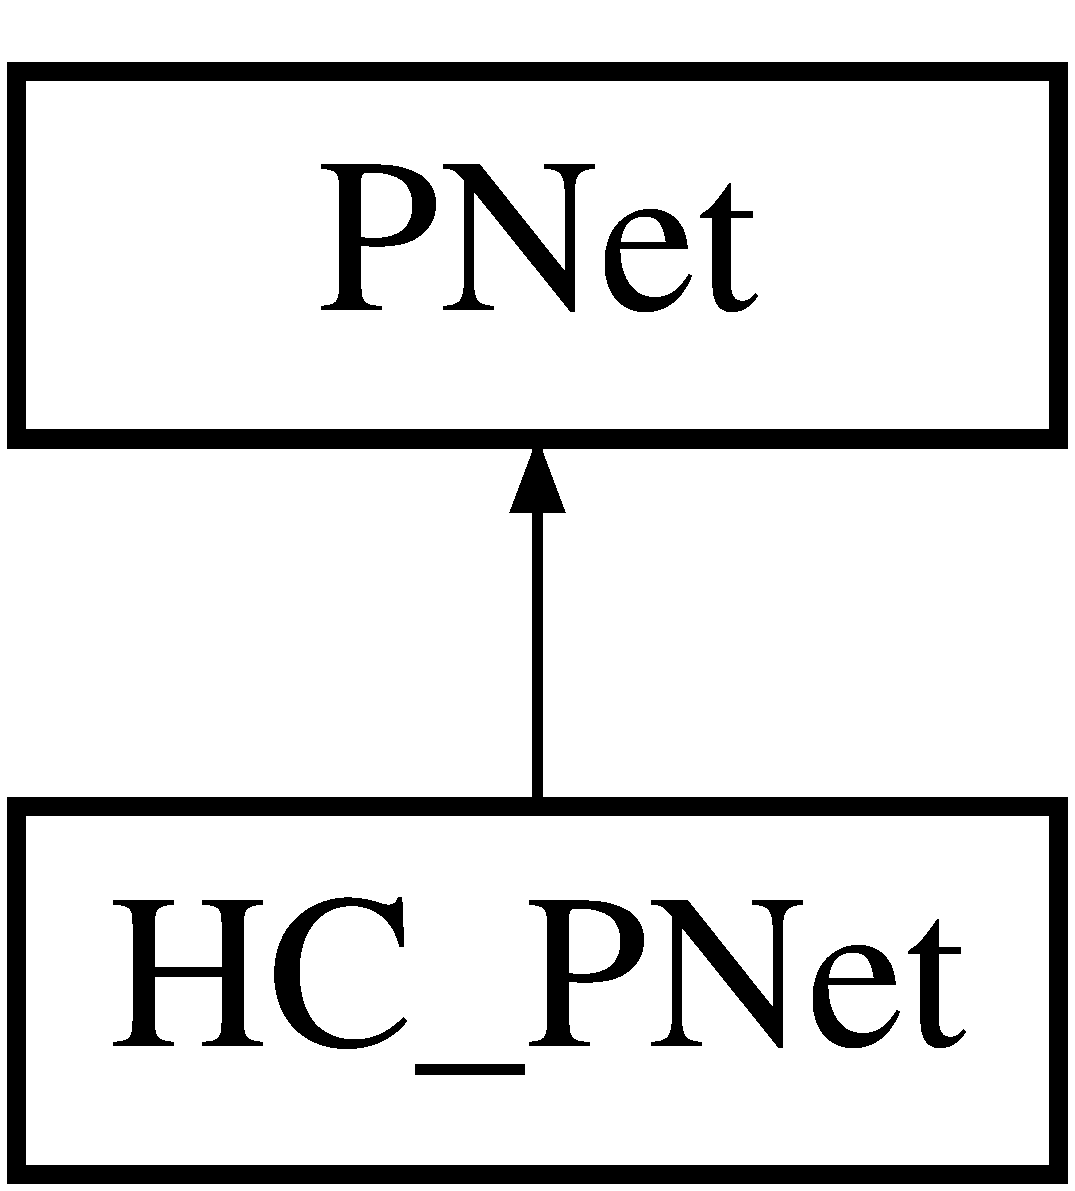
\includegraphics[height=2.000000cm]{classHC__PNet}
\end{center}
\end{figure}
\subsection*{Public Member Functions}
\begin{DoxyCompactItemize}
\item 
{\bfseries H\+C\+\_\+\+P\+Net} (const int \&N, const int \&\hyperlink{classHC__PNet_a40f377e7056967c60f966101eb986035}{C}, const int \&\hyperlink{classHC__PNet_a059016e26712e4fd5f6fdbdc6a41ce79}{S})\hypertarget{classHC__PNet_a5c7aca1e9fa59ca5aee29894de0b970f}{}\label{classHC__PNet_a5c7aca1e9fa59ca5aee29894de0b970f}

\item 
void {\bfseries import\+\_\+connections} (const std\+::string \&filename)\hypertarget{classHC__PNet_a91cd9aaa6acbf80f6dcca26ba1e5cd4f}{}\label{classHC__PNet_a91cd9aaa6acbf80f6dcca26ba1e5cd4f}

\item 
void {\bfseries print\+\_\+cm} ()\hypertarget{classHC__PNet_a49ff9fe01c408c0c028d736135dd4ef3}{}\label{classHC__PNet_a49ff9fe01c408c0c028d736135dd4ef3}

\item 
void {\bfseries save\+\_\+states\+\_\+to\+\_\+file} (const std\+::string \&filename)\hypertarget{classHC__PNet_a0f1e9277e2f5320ff638c9d6adf7c1db}{}\label{classHC__PNet_a0f1e9277e2f5320ff638c9d6adf7c1db}

\item 
void {\bfseries save\+\_\+connections\+\_\+to\+\_\+file} (const std\+::string \&filename)\hypertarget{classHC__PNet_a7d72eed734dc1a8c42f760db4ce19f0a}{}\label{classHC__PNet_a7d72eed734dc1a8c42f760db4ce19f0a}

\item 
void {\bfseries save\+\_\+\+J\+\_\+to\+\_\+file} (const std\+::string \&filename)\hypertarget{classHC__PNet_aaf22bc06a174cbe262a0ddbceb8cb079}{}\label{classHC__PNet_aaf22bc06a174cbe262a0ddbceb8cb079}

\item 
void {\bfseries connect\+\_\+units} (std\+::default\+\_\+random\+\_\+engine \&generator)\hypertarget{classHC__PNet_a404e5bb38475c42180d615e2dda8418d}{}\label{classHC__PNet_a404e5bb38475c42180d615e2dda8418d}

\item 
void {\bfseries init\+\_\+network} (const \+\_\+\+\_\+fpv \&beta, const \+\_\+\+\_\+fpv \&U, const int \&p, const \+\_\+\+\_\+fpv \&a, const int $\ast$xi)\hypertarget{classHC__PNet_afff5ec340c4a16084b2d8668a3c96a2f}{}\label{classHC__PNet_afff5ec340c4a16084b2d8668a3c96a2f}

\item 
void {\bfseries start\+\_\+dynamics} (std\+::default\+\_\+random\+\_\+engine \&generator, const int \&p, const int \&tstatus, const int \&nupdates, const int $\ast$xi, const int \&pattern, const \+\_\+\+\_\+fpv \&a, const \+\_\+\+\_\+fpv \&U, const \+\_\+\+\_\+fpv \&w, const \+\_\+\+\_\+fpv \&g, const \+\_\+\+\_\+fpv \&tau, const \+\_\+\+\_\+fpv \&b1, const \+\_\+\+\_\+fpv \&b2, const \+\_\+\+\_\+fpv \&b3, const \+\_\+\+\_\+fpv \&beta, const int \&tx)\hypertarget{classHC__PNet_a23cc68c5ef1225dddda2e3b5f11f5d80}{}\label{classHC__PNet_a23cc68c5ef1225dddda2e3b5f11f5d80}

\end{DoxyCompactItemize}
\subsection*{Private Member Functions}
\begin{DoxyCompactItemize}
\item 
void {\bfseries init\+\_\+states} (const \+\_\+\+\_\+fpv \&beta, const \+\_\+\+\_\+fpv \&U)\hypertarget{classHC__PNet_ac0b0fa614dced55cd174a75760c433a6}{}\label{classHC__PNet_ac0b0fa614dced55cd174a75760c433a6}

\item 
void {\bfseries update\+\_\+rule} (const int \&unit, const int \&pattern, const \+\_\+\+\_\+fpv \&U, const \+\_\+\+\_\+fpv \&w, const \+\_\+\+\_\+fpv \&g, const \+\_\+\+\_\+fpv \&tau, const \+\_\+\+\_\+fpv \&b1, const \+\_\+\+\_\+fpv \&b2, const \+\_\+\+\_\+fpv \&b3, const \+\_\+\+\_\+fpv \&beta, const int \&tx, const int \&t)\hypertarget{classHC__PNet_aa52cb9b21bafd7d988a7f436ab374713}{}\label{classHC__PNet_aa52cb9b21bafd7d988a7f436ab374713}

\item 
void {\bfseries evaluate\+\_\+m} (const int \&p, const \+\_\+\+\_\+fpv \&a, const int $\ast$xi, \+\_\+\+\_\+fpv m\mbox{[}$\,$\mbox{]})\hypertarget{classHC__PNet_a98650ec17421ae816d27d897149d511e}{}\label{classHC__PNet_a98650ec17421ae816d27d897149d511e}

\item 
void {\bfseries init\+\_\+J} (const int \&p, const \+\_\+\+\_\+fpv \&a, const int $\ast$xi)\hypertarget{classHC__PNet_a44f9724a29ab7c518438dc3c15c59204}{}\label{classHC__PNet_a44f9724a29ab7c518438dc3c15c59204}

\end{DoxyCompactItemize}
\subsection*{Private Attributes}
\begin{DoxyCompactItemize}
\item 
int \hyperlink{classHC__PNet_a40f377e7056967c60f966101eb986035}{C}
\item 
int \hyperlink{classHC__PNet_a059016e26712e4fd5f6fdbdc6a41ce79}{S}
\item 
int $\ast$ \hyperlink{classHC__PNet_a151d918ab156eda6394ecea56aa1b513}{cm}
\item 
\+\_\+\+\_\+fpv $\ast$ \hyperlink{classHC__PNet_a30c13f798fbcea6d617d09e8f06b7151}{J}
\item 
\+\_\+\+\_\+fpv $\ast$ {\bfseries active\+\_\+states}\hypertarget{classHC__PNet_a9b061bd0e3d89e46f6fabe253fc316fd}{}\label{classHC__PNet_a9b061bd0e3d89e46f6fabe253fc316fd}

\item 
\+\_\+\+\_\+fpv $\ast$ {\bfseries inactive\+\_\+states}\hypertarget{classHC__PNet_a37532e104b8ee801f3a344b68f30109c}{}\label{classHC__PNet_a37532e104b8ee801f3a344b68f30109c}

\item 
int $\ast$ {\bfseries ucm}\hypertarget{classHC__PNet_aa6a29609c184eb93f6f69aa97ed249a0}{}\label{classHC__PNet_aa6a29609c184eb93f6f69aa97ed249a0}

\item 
\+\_\+\+\_\+fpv $\ast$ {\bfseries active\+\_\+r}\hypertarget{classHC__PNet_a91d677edd2ce9a575eaefb2577263b58}{}\label{classHC__PNet_a91d677edd2ce9a575eaefb2577263b58}

\item 
\+\_\+\+\_\+fpv $\ast$ {\bfseries inactive\+\_\+r}\hypertarget{classHC__PNet_a7983d6b96e063925a3a625a3af197802}{}\label{classHC__PNet_a7983d6b96e063925a3a625a3af197802}

\item 
\+\_\+\+\_\+fpv $\ast$ {\bfseries h}\hypertarget{classHC__PNet_a68c66f7d4be2a581fd7f1ef6832ce894}{}\label{classHC__PNet_a68c66f7d4be2a581fd7f1ef6832ce894}

\item 
\+\_\+\+\_\+fpv $\ast$ {\bfseries theta}\hypertarget{classHC__PNet_a757db271f29e1b6a720cf59603c02ab5}{}\label{classHC__PNet_a757db271f29e1b6a720cf59603c02ab5}

\item 
int $\ast$ {\bfseries xi}\hypertarget{classHC__PNet_ad396474173f31c5f4cc3e94d0beb1ed6}{}\label{classHC__PNet_ad396474173f31c5f4cc3e94d0beb1ed6}

\end{DoxyCompactItemize}
\subsection*{Additional Inherited Members}


\subsection{Detailed Description}
Class defining the High connectivity network 

\subsection{Member Data Documentation}
\index{H\+C\+\_\+\+P\+Net@{H\+C\+\_\+\+P\+Net}!C@{C}}
\index{C@{C}!H\+C\+\_\+\+P\+Net@{H\+C\+\_\+\+P\+Net}}
\subsubsection[{\texorpdfstring{C}{C}}]{\setlength{\rightskip}{0pt plus 5cm}int H\+C\+\_\+\+P\+Net\+::C\hspace{0.3cm}{\ttfamily [private]}}\hypertarget{classHC__PNet_a40f377e7056967c60f966101eb986035}{}\label{classHC__PNet_a40f377e7056967c60f966101eb986035}
Number of connections per unit \index{H\+C\+\_\+\+P\+Net@{H\+C\+\_\+\+P\+Net}!cm@{cm}}
\index{cm@{cm}!H\+C\+\_\+\+P\+Net@{H\+C\+\_\+\+P\+Net}}
\subsubsection[{\texorpdfstring{cm}{cm}}]{\setlength{\rightskip}{0pt plus 5cm}int$\ast$ H\+C\+\_\+\+P\+Net\+::cm\hspace{0.3cm}{\ttfamily [private]}}\hypertarget{classHC__PNet_a151d918ab156eda6394ecea56aa1b513}{}\label{classHC__PNet_a151d918ab156eda6394ecea56aa1b513}
Connectivity matrix \index{H\+C\+\_\+\+P\+Net@{H\+C\+\_\+\+P\+Net}!J@{J}}
\index{J@{J}!H\+C\+\_\+\+P\+Net@{H\+C\+\_\+\+P\+Net}}
\subsubsection[{\texorpdfstring{J}{J}}]{\setlength{\rightskip}{0pt plus 5cm}\+\_\+\+\_\+fpv$\ast$ H\+C\+\_\+\+P\+Net\+::J\hspace{0.3cm}{\ttfamily [private]}}\hypertarget{classHC__PNet_a30c13f798fbcea6d617d09e8f06b7151}{}\label{classHC__PNet_a30c13f798fbcea6d617d09e8f06b7151}
J tensor \index{H\+C\+\_\+\+P\+Net@{H\+C\+\_\+\+P\+Net}!S@{S}}
\index{S@{S}!H\+C\+\_\+\+P\+Net@{H\+C\+\_\+\+P\+Net}}
\subsubsection[{\texorpdfstring{S}{S}}]{\setlength{\rightskip}{0pt plus 5cm}int H\+C\+\_\+\+P\+Net\+::S\hspace{0.3cm}{\ttfamily [private]}}\hypertarget{classHC__PNet_a059016e26712e4fd5f6fdbdc6a41ce79}{}\label{classHC__PNet_a059016e26712e4fd5f6fdbdc6a41ce79}
Number of states per unit 

The documentation for this class was generated from the following files\+:\begin{DoxyCompactItemize}
\item 
/home/deathquasar/\+Projects/\+M\+H\+P\+C/\+Thesis/\+Code/\+Potts\+\_\+code/include/hc\+\_\+pnet.\+h\item 
/home/deathquasar/\+Projects/\+M\+H\+P\+C/\+Thesis/\+Code/\+Potts\+\_\+code/lib/hc\+\_\+pnet.\+cpp\end{DoxyCompactItemize}

\hypertarget{classLC__PNet}{}\section{L\+C\+\_\+\+P\+Net Class Reference}
\label{classLC__PNet}\index{L\+C\+\_\+\+P\+Net@{L\+C\+\_\+\+P\+Net}}
Inheritance diagram for L\+C\+\_\+\+P\+Net\+:\begin{figure}[H]
\begin{center}
\leavevmode
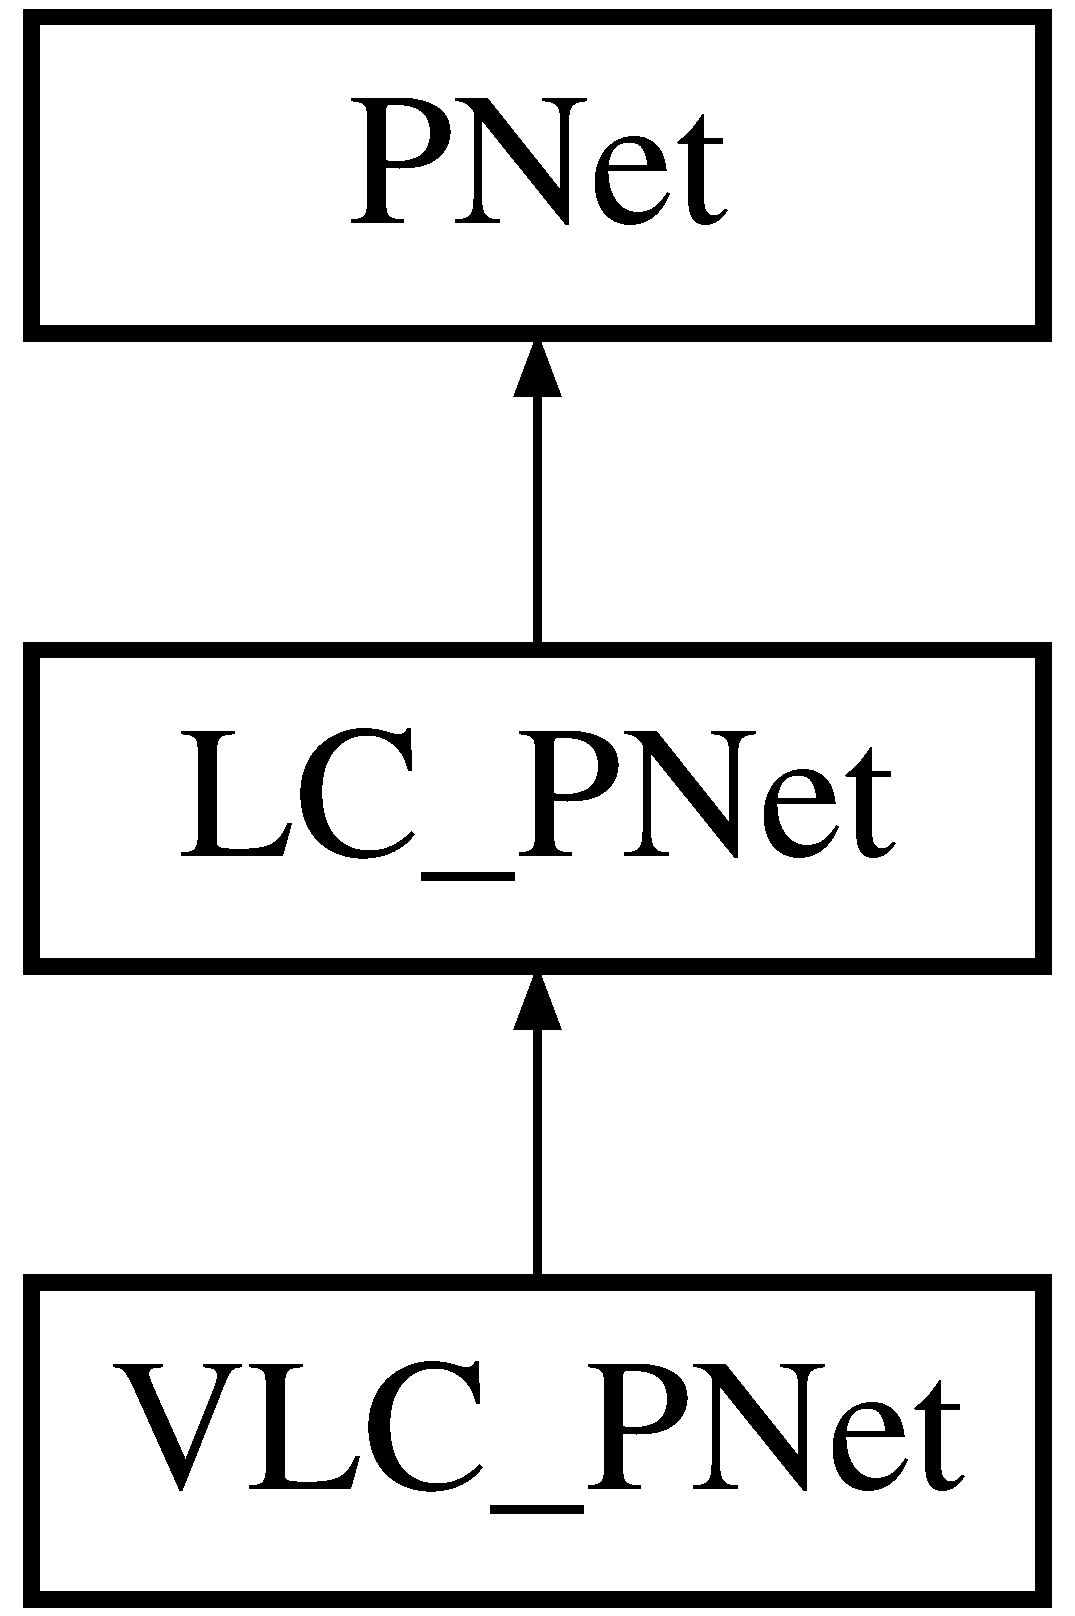
\includegraphics[height=3.000000cm]{classLC__PNet}
\end{center}
\end{figure}
\subsection*{Public Member Functions}
\begin{DoxyCompactItemize}
\item 
\hyperlink{classLC__PNet_a24f5b64eb7d135f812b05cfe747ddcc3}{L\+C\+\_\+\+P\+Net} (const int \&N, const int \&C, const int \&S)
\item 
void {\bfseries import\+\_\+connections} (const std\+::string \&filename)\hypertarget{classLC__PNet_a699f289ae423aa2af17139502654ab81}{}\label{classLC__PNet_a699f289ae423aa2af17139502654ab81}

\item 
void {\bfseries print\+\_\+cm} ()\hypertarget{classLC__PNet_afedba98cfd4a57742b963bf1fefdebed}{}\label{classLC__PNet_afedba98cfd4a57742b963bf1fefdebed}

\item 
void {\bfseries save\+\_\+states\+\_\+to\+\_\+file} (const std\+::string \&filename)\hypertarget{classLC__PNet_ac66589462b8882839a7a9849ce2025fa}{}\label{classLC__PNet_ac66589462b8882839a7a9849ce2025fa}

\item 
void {\bfseries save\+\_\+connections\+\_\+to\+\_\+file} (const std\+::string \&filename)\hypertarget{classLC__PNet_a1a66a51c4b649d64812d8c7eb49bda56}{}\label{classLC__PNet_a1a66a51c4b649d64812d8c7eb49bda56}

\item 
void {\bfseries save\+\_\+\+J\+\_\+to\+\_\+file} (const std\+::string \&filename)\hypertarget{classLC__PNet_afef840ecfc8b5b3a9180ca3c8e7f821f}{}\label{classLC__PNet_afef840ecfc8b5b3a9180ca3c8e7f821f}

\item 
void {\bfseries connect\+\_\+units} (std\+::default\+\_\+random\+\_\+engine \&generator)\hypertarget{classLC__PNet_ab9a618c5fc495ee199b420d0aa16758a}{}\label{classLC__PNet_ab9a618c5fc495ee199b420d0aa16758a}

\item 
void {\bfseries init\+\_\+network} (const \+\_\+\+\_\+fpv \&beta, const \+\_\+\+\_\+fpv \&U, const int \&p, const \+\_\+\+\_\+fpv \&a, const int $\ast$xi)\hypertarget{classLC__PNet_a0308d587505adab982a9e4322b8ac9ba}{}\label{classLC__PNet_a0308d587505adab982a9e4322b8ac9ba}

\item 
void {\bfseries start\+\_\+dynamics} (std\+::default\+\_\+random\+\_\+engine \&generator, const int \&p, const int \&tstatus, const int \&nupdates, const int $\ast$xi, const int \&pattern, const \+\_\+\+\_\+fpv \&a, const \+\_\+\+\_\+fpv \&U, const \+\_\+\+\_\+fpv \&w, const \+\_\+\+\_\+fpv \&g, const \+\_\+\+\_\+fpv \&tau, const \+\_\+\+\_\+fpv \&b1, const \+\_\+\+\_\+fpv \&b2, const \+\_\+\+\_\+fpv \&b3, const \+\_\+\+\_\+fpv \&beta, const int \&tx)\hypertarget{classLC__PNet_adadf57b63af5fc9238bb97df3b56381d}{}\label{classLC__PNet_adadf57b63af5fc9238bb97df3b56381d}

\end{DoxyCompactItemize}
\subsection*{Protected Member Functions}
\begin{DoxyCompactItemize}
\item 
void {\bfseries init\+\_\+states} (const \+\_\+\+\_\+fpv \&beta, const \+\_\+\+\_\+fpv \&U)\hypertarget{classLC__PNet_a2925dc1c225646f4be3e466383812f14}{}\label{classLC__PNet_a2925dc1c225646f4be3e466383812f14}

\item 
void {\bfseries update\+\_\+rule} (const int \&unit, const \+\_\+\+\_\+fpv buffer\mbox{[}$\,$\mbox{]}, const int \&pattern, const \+\_\+\+\_\+fpv \&U, const \+\_\+\+\_\+fpv \&w, const \+\_\+\+\_\+fpv \&g, const \+\_\+\+\_\+fpv \&tau, const \+\_\+\+\_\+fpv \&b1, const \+\_\+\+\_\+fpv \&b2, const \+\_\+\+\_\+fpv \&b3, const \+\_\+\+\_\+fpv \&beta, const int \&tx, const int \&t)\hypertarget{classLC__PNet_aef7091aa9525fb95c3f1df19f801b535}{}\label{classLC__PNet_aef7091aa9525fb95c3f1df19f801b535}

\item 
void {\bfseries evaluate\+\_\+m} (const int \&p, const \+\_\+\+\_\+fpv \&a, const int $\ast$xi, \+\_\+\+\_\+fpv m\mbox{[}$\,$\mbox{]})\hypertarget{classLC__PNet_a184fb2c6b021c7a814954e9750347b1c}{}\label{classLC__PNet_a184fb2c6b021c7a814954e9750347b1c}

\item 
void {\bfseries init\+\_\+J} (const int \&p, const \+\_\+\+\_\+fpv \&a, const int $\ast$xi)\hypertarget{classLC__PNet_a22278003507e1871152e4024002a7ff9}{}\label{classLC__PNet_a22278003507e1871152e4024002a7ff9}

\end{DoxyCompactItemize}
\subsection*{Protected Attributes}
\begin{DoxyCompactItemize}
\item 
int {\bfseries C}\hypertarget{classLC__PNet_ac6fbf61a77df3fefd1add38665e7b717}{}\label{classLC__PNet_ac6fbf61a77df3fefd1add38665e7b717}

\item 
int {\bfseries S}\hypertarget{classLC__PNet_ab6a71cf2a87d2a84ef26d63da7cb28c7}{}\label{classLC__PNet_ab6a71cf2a87d2a84ef26d63da7cb28c7}

\item 
int $\ast$ {\bfseries cm}\hypertarget{classLC__PNet_a4d5e6bfeff710d069640abaabf92e9d8}{}\label{classLC__PNet_a4d5e6bfeff710d069640abaabf92e9d8}

\item 
\+\_\+\+\_\+fpv $\ast$ {\bfseries J}\hypertarget{classLC__PNet_a07424445de5664c7840fa76867d01491}{}\label{classLC__PNet_a07424445de5664c7840fa76867d01491}

\item 
\+\_\+\+\_\+fpv $\ast$ {\bfseries active\+\_\+states}\hypertarget{classLC__PNet_a4c085a26d4bc5cc9c048f5652bf7d3c7}{}\label{classLC__PNet_a4c085a26d4bc5cc9c048f5652bf7d3c7}

\item 
\+\_\+\+\_\+fpv $\ast$ {\bfseries inactive\+\_\+states}\hypertarget{classLC__PNet_aa286239886cffadfb0098b4af9391cfd}{}\label{classLC__PNet_aa286239886cffadfb0098b4af9391cfd}

\item 
int $\ast$ {\bfseries ucm}\hypertarget{classLC__PNet_af1e4cb3b01d9eea8dc4ee932ac486f5f}{}\label{classLC__PNet_af1e4cb3b01d9eea8dc4ee932ac486f5f}

\item 
\+\_\+\+\_\+fpv $\ast$ {\bfseries active\+\_\+r}\hypertarget{classLC__PNet_a232191ada434e427069b9d73a32c6c11}{}\label{classLC__PNet_a232191ada434e427069b9d73a32c6c11}

\item 
\+\_\+\+\_\+fpv $\ast$ {\bfseries inactive\+\_\+r}\hypertarget{classLC__PNet_a4eefb8f8377ce107099d63bbc3b129bf}{}\label{classLC__PNet_a4eefb8f8377ce107099d63bbc3b129bf}

\item 
\+\_\+\+\_\+fpv $\ast$ {\bfseries h}\hypertarget{classLC__PNet_a0f89876853795e0366d6f771295ec785}{}\label{classLC__PNet_a0f89876853795e0366d6f771295ec785}

\item 
\+\_\+\+\_\+fpv $\ast$ {\bfseries theta}\hypertarget{classLC__PNet_ab4352d5dd32171b45a3471be0de07a77}{}\label{classLC__PNet_ab4352d5dd32171b45a3471be0de07a77}

\item 
int $\ast$ {\bfseries xi}\hypertarget{classLC__PNet_ade19ecf3ac391db683a740bde9fde66b}{}\label{classLC__PNet_ade19ecf3ac391db683a740bde9fde66b}

\end{DoxyCompactItemize}
\subsection*{Additional Inherited Members}


\subsection{Constructor \& Destructor Documentation}
\index{L\+C\+\_\+\+P\+Net@{L\+C\+\_\+\+P\+Net}!L\+C\+\_\+\+P\+Net@{L\+C\+\_\+\+P\+Net}}
\index{L\+C\+\_\+\+P\+Net@{L\+C\+\_\+\+P\+Net}!L\+C\+\_\+\+P\+Net@{L\+C\+\_\+\+P\+Net}}
\subsubsection[{\texorpdfstring{L\+C\+\_\+\+P\+Net(const int \&\+N, const int \&\+C, const int \&\+S)}{LC_PNet(const int &N, const int &C, const int &S)}}]{\setlength{\rightskip}{0pt plus 5cm}L\+C\+\_\+\+P\+Net\+::\+L\+C\+\_\+\+P\+Net (
\begin{DoxyParamCaption}
\item[{const int \&}]{N, }
\item[{const int \&}]{C, }
\item[{const int \&}]{S}
\end{DoxyParamCaption}
)}\hypertarget{classLC__PNet_a24f5b64eb7d135f812b05cfe747ddcc3}{}\label{classLC__PNet_a24f5b64eb7d135f812b05cfe747ddcc3}
\char`\"{}£\char`\"{} 

The documentation for this class was generated from the following files\+:\begin{DoxyCompactItemize}
\item 
/home/deathquasar/\+Projects/\+M\+H\+P\+C/\+Thesis/\+Code/\+Potts\+\_\+code/include/lc\+\_\+pnet.\+h\item 
/home/deathquasar/\+Projects/\+M\+H\+P\+C/\+Thesis/\+Code/\+Potts\+\_\+code/lib/lc\+\_\+pnet.\+cpp\end{DoxyCompactItemize}

\hypertarget{structparameters}{}\section{parameters Struct Reference}
\label{structparameters}\index{parameters@{parameters}}
\subsection*{Public Attributes}
\begin{DoxyCompactItemize}
\item 
int {\bfseries N}\hypertarget{structparameters_a0b2132a2da84d48e4575f6d9e8e899ee}{}\label{structparameters_a0b2132a2da84d48e4575f6d9e8e899ee}

\item 
int {\bfseries C}\hypertarget{structparameters_a2143fd1bb0b1132240b2ac1f48797837}{}\label{structparameters_a2143fd1bb0b1132240b2ac1f48797837}

\item 
int {\bfseries p}\hypertarget{structparameters_a83fbd6f42d209aab6d3aa8360835cb55}{}\label{structparameters_a83fbd6f42d209aab6d3aa8360835cb55}

\item 
int {\bfseries S}\hypertarget{structparameters_a491bc36fe07cd5249f7d54fd82f7cb63}{}\label{structparameters_a491bc36fe07cd5249f7d54fd82f7cb63}

\item 
int {\bfseries nupdates}\hypertarget{structparameters_adaa744c06c33db9f1116ddd62bf97303}{}\label{structparameters_adaa744c06c33db9f1116ddd62bf97303}

\item 
int {\bfseries Num\+Set}\hypertarget{structparameters_a7308970e43d375353d1fccc1e581a8f4}{}\label{structparameters_a7308970e43d375353d1fccc1e581a8f4}

\item 
int {\bfseries N\+\_\+fact}\hypertarget{structparameters_a3fd36b05da1943711146096ac4528c92}{}\label{structparameters_a3fd36b05da1943711146096ac4528c92}

\item 
int {\bfseries Num\+\_\+fact}\hypertarget{structparameters_a9d567a9e2b598ee9fbe8ac4ecd611bb4}{}\label{structparameters_a9d567a9e2b598ee9fbe8ac4ecd611bb4}

\item 
int {\bfseries tstatus}\hypertarget{structparameters_ab1a47a209b6cbeea981c2001aa48a603}{}\label{structparameters_ab1a47a209b6cbeea981c2001aa48a603}

\item 
\+\_\+\+\_\+fpv {\bfseries a}\hypertarget{structparameters_a855416f306051d9fafd42310c4c39e79}{}\label{structparameters_a855416f306051d9fafd42310c4c39e79}

\item 
\+\_\+\+\_\+fpv {\bfseries U}\hypertarget{structparameters_afe57c1c9613decd31b31cbe63744ca3a}{}\label{structparameters_afe57c1c9613decd31b31cbe63744ca3a}

\item 
\+\_\+\+\_\+fpv {\bfseries b1}\hypertarget{structparameters_a98a51cfec1fecb74da95181555bbacba}{}\label{structparameters_a98a51cfec1fecb74da95181555bbacba}

\item 
\+\_\+\+\_\+fpv {\bfseries b2}\hypertarget{structparameters_a80d5e1baec765e78bbb55eb4623344a3}{}\label{structparameters_a80d5e1baec765e78bbb55eb4623344a3}

\item 
\+\_\+\+\_\+fpv {\bfseries b3}\hypertarget{structparameters_ab90f8477078e4e234b38c0a17c537d6d}{}\label{structparameters_ab90f8477078e4e234b38c0a17c537d6d}

\item 
\+\_\+\+\_\+fpv {\bfseries beta}\hypertarget{structparameters_a18029b953bec42c937a931ecb083cfa2}{}\label{structparameters_a18029b953bec42c937a931ecb083cfa2}

\item 
\+\_\+\+\_\+fpv {\bfseries w}\hypertarget{structparameters_ab95743b50344ac26c8b78bdebc1c37d8}{}\label{structparameters_ab95743b50344ac26c8b78bdebc1c37d8}

\item 
\+\_\+\+\_\+fpv {\bfseries g}\hypertarget{structparameters_aec758045deddba9c9c7cb20fc7998fdd}{}\label{structparameters_aec758045deddba9c9c7cb20fc7998fdd}

\item 
\+\_\+\+\_\+fpv {\bfseries tau}\hypertarget{structparameters_a665737e3c32140c9dd8e023723eb45ac}{}\label{structparameters_a665737e3c32140c9dd8e023723eb45ac}

\item 
\+\_\+\+\_\+fpv {\bfseries a\+\_\+fact}\hypertarget{structparameters_a98eb1f46f30452fd05f1836db2cd483f}{}\label{structparameters_a98eb1f46f30452fd05f1836db2cd483f}

\item 
\+\_\+\+\_\+fpv {\bfseries eps}\hypertarget{structparameters_a612546fcd2f7f8c78055fa5be1a27dcd}{}\label{structparameters_a612546fcd2f7f8c78055fa5be1a27dcd}

\item 
\+\_\+\+\_\+fpv {\bfseries a\+\_\+pf}\hypertarget{structparameters_a4f824daf21865bb4be9134614cb0df38}{}\label{structparameters_a4f824daf21865bb4be9134614cb0df38}

\item 
\+\_\+\+\_\+fpv {\bfseries fact\+\_\+eigen\+\_\+slope}\hypertarget{structparameters_af7ed1eca879710da4d7521e6b14a5da2}{}\label{structparameters_af7ed1eca879710da4d7521e6b14a5da2}

\end{DoxyCompactItemize}


The documentation for this struct was generated from the following file\+:\begin{DoxyCompactItemize}
\item 
/home/deathquasar/\+Projects/\+M\+H\+P\+C/\+Thesis/\+Code/\+Potts\+\_\+code/include/parameters\+\_\+struct.\+h\end{DoxyCompactItemize}

\hypertarget{classPatternGen}{}\section{Pattern\+Gen Class Reference}
\label{classPatternGen}\index{Pattern\+Gen@{Pattern\+Gen}}
\subsection*{Public Member Functions}
\begin{DoxyCompactItemize}
\item 
{\bfseries Pattern\+Gen} (const int N, const int p, const int S, const \+\_\+\+\_\+fpv a, const \+\_\+\+\_\+fpv beta, const int N\+\_\+fact, const int Num\+\_\+fact, const \+\_\+\+\_\+fpv a\+\_\+fact, const \+\_\+\+\_\+fpv eps, const \+\_\+\+\_\+fpv a\+\_\+pf, const \+\_\+\+\_\+fpv fact\+\_\+eigen\+\_\+slope)\hypertarget{classPatternGen_ae347681b782de3d3b415f5e0212c687c}{}\label{classPatternGen_ae347681b782de3d3b415f5e0212c687c}

\item 
void {\bfseries generate} ()\hypertarget{classPatternGen_a1e77dc569b771ee5185f51c7ca900e1a}{}\label{classPatternGen_a1e77dc569b771ee5185f51c7ca900e1a}

\item 
void {\bfseries eval\+\_\+stats} ()\hypertarget{classPatternGen_ace5ff5d0cb3ccc4b8b4941a22096dbc2}{}\label{classPatternGen_ace5ff5d0cb3ccc4b8b4941a22096dbc2}

\item 
void {\bfseries save\+\_\+pattern\+\_\+to\+\_\+file} (const std\+::string filename)\hypertarget{classPatternGen_ae33872117e255a8db86ea50d1a9cb413}{}\label{classPatternGen_ae33872117e255a8db86ea50d1a9cb413}

\item 
int $\ast$ {\bfseries get\+\_\+patt} ()\hypertarget{classPatternGen_a4c3e875c5a117b4fd3de9a83bc396df8}{}\label{classPatternGen_a4c3e875c5a117b4fd3de9a83bc396df8}

\item 
int $\ast$ {\bfseries get\+\_\+patt} (const int n)\hypertarget{classPatternGen_aaceb7c87b9efea67ba77ca78e2352bae}{}\label{classPatternGen_aaceb7c87b9efea67ba77ca78e2352bae}

\end{DoxyCompactItemize}
\subsection*{Private Attributes}
\begin{DoxyCompactItemize}
\item 
int {\bfseries N}\hypertarget{classPatternGen_a863ddbe22dd40007c627c1b832ccf37e}{}\label{classPatternGen_a863ddbe22dd40007c627c1b832ccf37e}

\item 
int {\bfseries p}\hypertarget{classPatternGen_a8165d434665ed29849bc082d8be33645}{}\label{classPatternGen_a8165d434665ed29849bc082d8be33645}

\item 
int {\bfseries S}\hypertarget{classPatternGen_a2a3d575178652e5604e6ea58ae511e31}{}\label{classPatternGen_a2a3d575178652e5604e6ea58ae511e31}

\item 
\+\_\+\+\_\+fpv {\bfseries a}\hypertarget{classPatternGen_a732898973f15edb9f41f7ae11e5f0473}{}\label{classPatternGen_a732898973f15edb9f41f7ae11e5f0473}

\item 
\+\_\+\+\_\+fpv {\bfseries beta}\hypertarget{classPatternGen_ade3f26e89aec3a386855c2eb50a6d30c}{}\label{classPatternGen_ade3f26e89aec3a386855c2eb50a6d30c}

\item 
int {\bfseries N\+\_\+fact}\hypertarget{classPatternGen_a1e138ac8ad854a293490cc07bf943cbb}{}\label{classPatternGen_a1e138ac8ad854a293490cc07bf943cbb}

\item 
int {\bfseries Num\+\_\+fact}\hypertarget{classPatternGen_aca87deb674f64a3d62ff0977594556d1}{}\label{classPatternGen_aca87deb674f64a3d62ff0977594556d1}

\item 
\+\_\+\+\_\+fpv {\bfseries a\+\_\+fact}\hypertarget{classPatternGen_ac00b2dfa4eda179b2e6f7d7d54ddd54f}{}\label{classPatternGen_ac00b2dfa4eda179b2e6f7d7d54ddd54f}

\item 
\+\_\+\+\_\+fpv {\bfseries eps}\hypertarget{classPatternGen_ac37104402643f90264bd0187f7f14ac0}{}\label{classPatternGen_ac37104402643f90264bd0187f7f14ac0}

\item 
\+\_\+\+\_\+fpv {\bfseries a\+\_\+pf}\hypertarget{classPatternGen_af88c6c784e7b8bfa4b549df95a34f697}{}\label{classPatternGen_af88c6c784e7b8bfa4b549df95a34f697}

\item 
\+\_\+\+\_\+fpv {\bfseries fact\+\_\+eigen\+\_\+slope}\hypertarget{classPatternGen_aff25acb39430526e6c993466c9b62155}{}\label{classPatternGen_aff25acb39430526e6c993466c9b62155}

\item 
int $\ast$ {\bfseries Patt}\hypertarget{classPatternGen_a238bdf97e540c55f916769b95ffe48f1}{}\label{classPatternGen_a238bdf97e540c55f916769b95ffe48f1}

\end{DoxyCompactItemize}
\subsection*{Friends}
\begin{DoxyCompactItemize}
\item 
class {\bfseries P\+Network}\hypertarget{classPatternGen_af18c1bfc19f67a8a280667eb030fb0d2}{}\label{classPatternGen_af18c1bfc19f67a8a280667eb030fb0d2}

\end{DoxyCompactItemize}


The documentation for this class was generated from the following files\+:\begin{DoxyCompactItemize}
\item 
/home/deathquasar/\+Projects/\+M\+H\+P\+C/\+Thesis/\+Code/\+Potts\+\_\+code/include/pattern\+\_\+gen.\+h\item 
/home/deathquasar/\+Projects/\+M\+H\+P\+C/\+Thesis/\+Code/\+Potts\+\_\+code/lib/pattern\+\_\+gen.\+cpp\end{DoxyCompactItemize}

\hypertarget{classPNet}{}\section{P\+Net Class Reference}
\label{classPNet}\index{P\+Net@{P\+Net}}
Inheritance diagram for P\+Net\+:\begin{figure}[H]
\begin{center}
\leavevmode
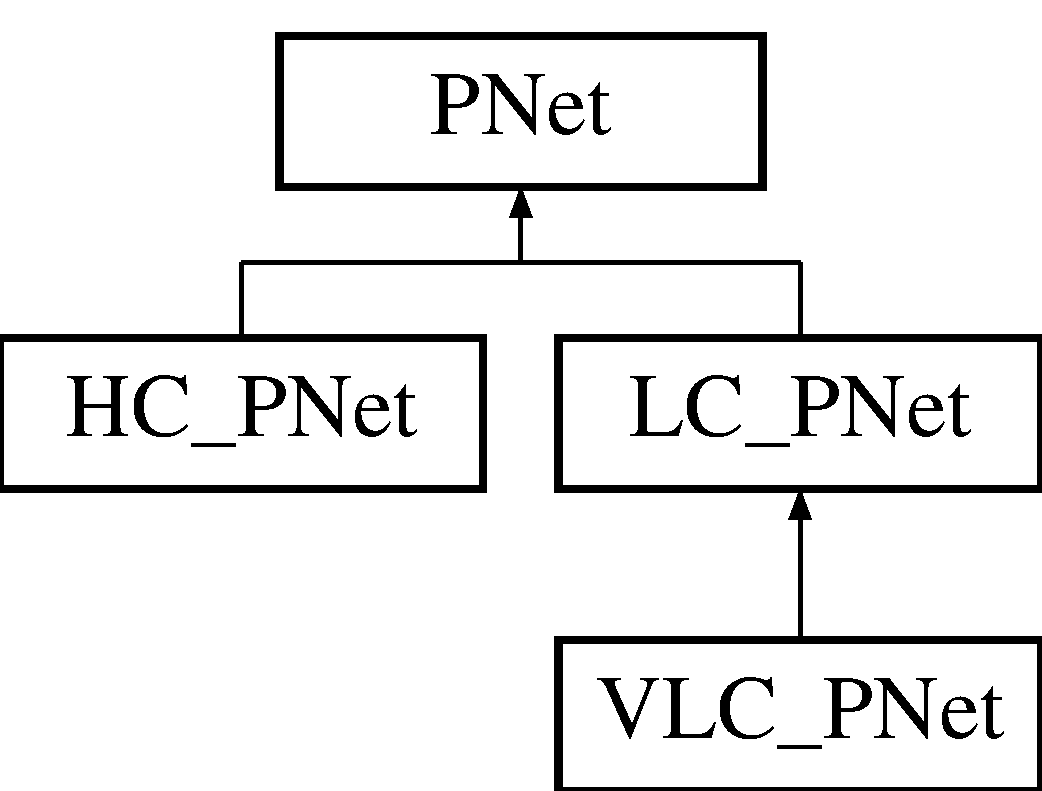
\includegraphics[height=3.000000cm]{classPNet}
\end{center}
\end{figure}
\subsection*{Public Member Functions}
\begin{DoxyCompactItemize}
\item 
{\bfseries P\+Net} (const int \&N)\hypertarget{classPNet_ae7bb66e9b6e3cc8bebf69f0acc467978}{}\label{classPNet_ae7bb66e9b6e3cc8bebf69f0acc467978}

\item 
void {\bfseries print\+\_\+ksequence} ()\hypertarget{classPNet_af8319c3b3ec476d5008df5fe45c3544d}{}\label{classPNet_af8319c3b3ec476d5008df5fe45c3544d}

\item 
virtual void {\bfseries print\+\_\+cm} ()=0\hypertarget{classPNet_a0f0c008ac7f00564bfdedfd3febd3602}{}\label{classPNet_a0f0c008ac7f00564bfdedfd3febd3602}

\item 
virtual void {\bfseries save\+\_\+states\+\_\+to\+\_\+file} (const std\+::string \&filename)=0\hypertarget{classPNet_a2cac2b992ff0b0520f5dbb1a029676b1}{}\label{classPNet_a2cac2b992ff0b0520f5dbb1a029676b1}

\item 
virtual void {\bfseries save\+\_\+connections\+\_\+to\+\_\+file} (const std\+::string \&filename)=0\hypertarget{classPNet_aad8dbda7540a1ed7d3fa142583770c0d}{}\label{classPNet_aad8dbda7540a1ed7d3fa142583770c0d}

\item 
virtual void {\bfseries save\+\_\+\+J\+\_\+to\+\_\+file} (const std\+::string \&filename)=0\hypertarget{classPNet_a98feeb763aa03d366e6bf5b05c240f25}{}\label{classPNet_a98feeb763aa03d366e6bf5b05c240f25}

\item 
virtual void {\bfseries init\+\_\+network} (const \+\_\+\+\_\+fpv \&beta, const \+\_\+\+\_\+fpv \&U, const int \&p, const \+\_\+\+\_\+fpv \&a, const int $\ast$xi)=0\hypertarget{classPNet_a63efd6e2d7c5a38e0a6ae77af655a405}{}\label{classPNet_a63efd6e2d7c5a38e0a6ae77af655a405}

\item 
virtual void {\bfseries start\+\_\+dynamics} (std\+::default\+\_\+random\+\_\+engine \&generator, const int \&p, const int \&tstatus, const int \&nupdates, const int $\ast$xi, const int \&pattern, const \+\_\+\+\_\+fpv \&a, const \+\_\+\+\_\+fpv \&U, const \+\_\+\+\_\+fpv \&w, const \+\_\+\+\_\+fpv \&g, const \+\_\+\+\_\+fpv \&tau, const \+\_\+\+\_\+fpv \&b1, const \+\_\+\+\_\+fpv \&b2, const \+\_\+\+\_\+fpv \&b3, const \+\_\+\+\_\+fpv \&beta, const int \&tx)=0\hypertarget{classPNet_afb427ff3050f26969782aec6bc76a5a7}{}\label{classPNet_afb427ff3050f26969782aec6bc76a5a7}

\end{DoxyCompactItemize}
\subsection*{Public Attributes}
\begin{DoxyCompactItemize}
\item 
\+\_\+\+\_\+fpv {\bfseries latching\+\_\+length}\hypertarget{classPNet_ac21a9a2f6de2fc6094bdfacc78142ffe}{}\label{classPNet_ac21a9a2f6de2fc6094bdfacc78142ffe}

\end{DoxyCompactItemize}
\subsection*{Protected Member Functions}
\begin{DoxyCompactItemize}
\item 
virtual void {\bfseries evaluate\+\_\+m} (const int \&p, const \+\_\+\+\_\+fpv \&a, const int $\ast$xi, \+\_\+\+\_\+fpv m\mbox{[}$\,$\mbox{]})=0\hypertarget{classPNet_a6d519b171b571fccbc1d263ff40822e3}{}\label{classPNet_a6d519b171b571fccbc1d263ff40822e3}

\item 
virtual void {\bfseries init\+\_\+J} (const int \&p, const \+\_\+\+\_\+fpv \&a, const int $\ast$xi)=0\hypertarget{classPNet_aeef297a15dc839818cd560228c9b8236}{}\label{classPNet_aeef297a15dc839818cd560228c9b8236}

\item 
void {\bfseries get\+\_\+status} (const int \&p, const int \&tx, const int \&t, const int $\ast$xi, const \+\_\+\+\_\+fpv \&a, int \&Mumaxold, int \&Mumax, int \&steps, bool \&stop)\hypertarget{classPNet_a3c22be54795d659f2ebab3725ad93946}{}\label{classPNet_a3c22be54795d659f2ebab3725ad93946}

\end{DoxyCompactItemize}
\subsection*{Protected Attributes}
\begin{DoxyCompactItemize}
\item 
int {\bfseries N}\hypertarget{classPNet_a165f64c0fb771ebbcb5851b27373cf30}{}\label{classPNet_a165f64c0fb771ebbcb5851b27373cf30}

\item 
std\+::vector$<$ int $>$ {\bfseries ksequence}\hypertarget{classPNet_ab636bd102fd68c5801c1b907dba52e9d}{}\label{classPNet_ab636bd102fd68c5801c1b907dba52e9d}

\end{DoxyCompactItemize}


The documentation for this class was generated from the following files\+:\begin{DoxyCompactItemize}
\item 
/home/deathquasar/\+Projects/\+M\+H\+P\+C/\+Thesis/\+Code/\+Potts\+\_\+code/lib/pnet.\+h\item 
/home/deathquasar/\+Projects/\+M\+H\+P\+C/\+Thesis/\+Code/\+Potts\+\_\+code/lib/pnet.\+cpp\end{DoxyCompactItemize}

\hypertarget{classPPS}{}\section{P\+PS Class Reference}
\label{classPPS}\index{P\+PS@{P\+PS}}
\subsection*{Static Public Member Functions}
\begin{DoxyCompactItemize}
\item 
static void {\bfseries start} ()\hypertarget{classPPS_a25cae7ae5a03f02d8c44b2b9b163ebe6}{}\label{classPPS_a25cae7ae5a03f02d8c44b2b9b163ebe6}

\end{DoxyCompactItemize}
\subsection*{Static Public Attributes}
\begin{DoxyCompactItemize}
\item 
static int {\bfseries pid}\hypertarget{classPPS_a4e924fe2bb5ac2451243e7adc4f943ef}{}\label{classPPS_a4e924fe2bb5ac2451243e7adc4f943ef}

\item 
static int {\bfseries comm\+\_\+size}\hypertarget{classPPS_a499131be4386ab41cf334cf42170518e}{}\label{classPPS_a499131be4386ab41cf334cf42170518e}

\item 
static std\+::vector$<$ \hyperlink{structparameters}{parameters} $>$ {\bfseries plist}\hypertarget{classPPS_a0e5dcc27effd740a9d7b8d65356b80c1}{}\label{classPPS_a0e5dcc27effd740a9d7b8d65356b80c1}

\end{DoxyCompactItemize}


The documentation for this class was generated from the following files\+:\begin{DoxyCompactItemize}
\item 
/home/deathquasar/\+Projects/\+M\+H\+P\+C/\+Thesis/\+Code/\+Potts\+\_\+code/include/parallel\+\_\+scheduler.\+h\item 
/home/deathquasar/\+Projects/\+M\+H\+P\+C/\+Thesis/\+Code/\+Potts\+\_\+code/lib/parallel\+\_\+scheduler.\+cpp\end{DoxyCompactItemize}

\hypertarget{classRandomSequence}{}\section{Random\+Sequence Class Reference}
\label{classRandomSequence}\index{Random\+Sequence@{Random\+Sequence}}
\subsection*{Public Member Functions}
\begin{DoxyCompactItemize}
\item 
{\bfseries Random\+Sequence} (const int N)\hypertarget{classRandomSequence_a010f044bbdf4e8be029ba7b936e5c7ae}{}\label{classRandomSequence_a010f044bbdf4e8be029ba7b936e5c7ae}

\item 
void {\bfseries shuffle} (std\+::default\+\_\+random\+\_\+engine \&generator)\hypertarget{classRandomSequence_ab6ca117e2c7d36bdcf4b808c4c9a4e3e}{}\label{classRandomSequence_ab6ca117e2c7d36bdcf4b808c4c9a4e3e}

\item 
void {\bfseries print} ()\hypertarget{classRandomSequence_acf065adaf2b78987d23187bdd60081f0}{}\label{classRandomSequence_acf065adaf2b78987d23187bdd60081f0}

\item 
int $\ast$ {\bfseries begin} ()\hypertarget{classRandomSequence_ac2483da3051c252afe0fcc0c703774c5}{}\label{classRandomSequence_ac2483da3051c252afe0fcc0c703774c5}

\item 
int $\ast$ {\bfseries end} ()\hypertarget{classRandomSequence_a457062d456d29e8d8acbbe78f3a964db}{}\label{classRandomSequence_a457062d456d29e8d8acbbe78f3a964db}

\item 
int {\bfseries get} (const int \&i)\hypertarget{classRandomSequence_a87bbb74fa6a1b4f7c4e1bd07f011c724}{}\label{classRandomSequence_a87bbb74fa6a1b4f7c4e1bd07f011c724}

\end{DoxyCompactItemize}
\subsection*{Private Attributes}
\begin{DoxyCompactItemize}
\item 
int $\ast$ {\bfseries sequence}\hypertarget{classRandomSequence_ac2abe360115973753daaf9404bcb1b01}{}\label{classRandomSequence_ac2abe360115973753daaf9404bcb1b01}

\item 
int {\bfseries N}\hypertarget{classRandomSequence_ae18913047e907399b76ff6ffb4806c92}{}\label{classRandomSequence_ae18913047e907399b76ff6ffb4806c92}

\end{DoxyCompactItemize}


The documentation for this class was generated from the following files\+:\begin{DoxyCompactItemize}
\item 
/home/deathquasar/\+Projects/\+M\+H\+P\+C/\+Thesis/\+Code/\+Potts\+\_\+code/include/random\+\_\+seq.\+h\item 
/home/deathquasar/\+Projects/\+M\+H\+P\+C/\+Thesis/\+Code/\+Potts\+\_\+code/lib/random\+\_\+seq.\+cpp\end{DoxyCompactItemize}

\hypertarget{classVLC__PNet}{}\section{V\+L\+C\+\_\+\+P\+Net Class Reference}
\label{classVLC__PNet}\index{V\+L\+C\+\_\+\+P\+Net@{V\+L\+C\+\_\+\+P\+Net}}
Inheritance diagram for V\+L\+C\+\_\+\+P\+Net\+:\begin{figure}[H]
\begin{center}
\leavevmode
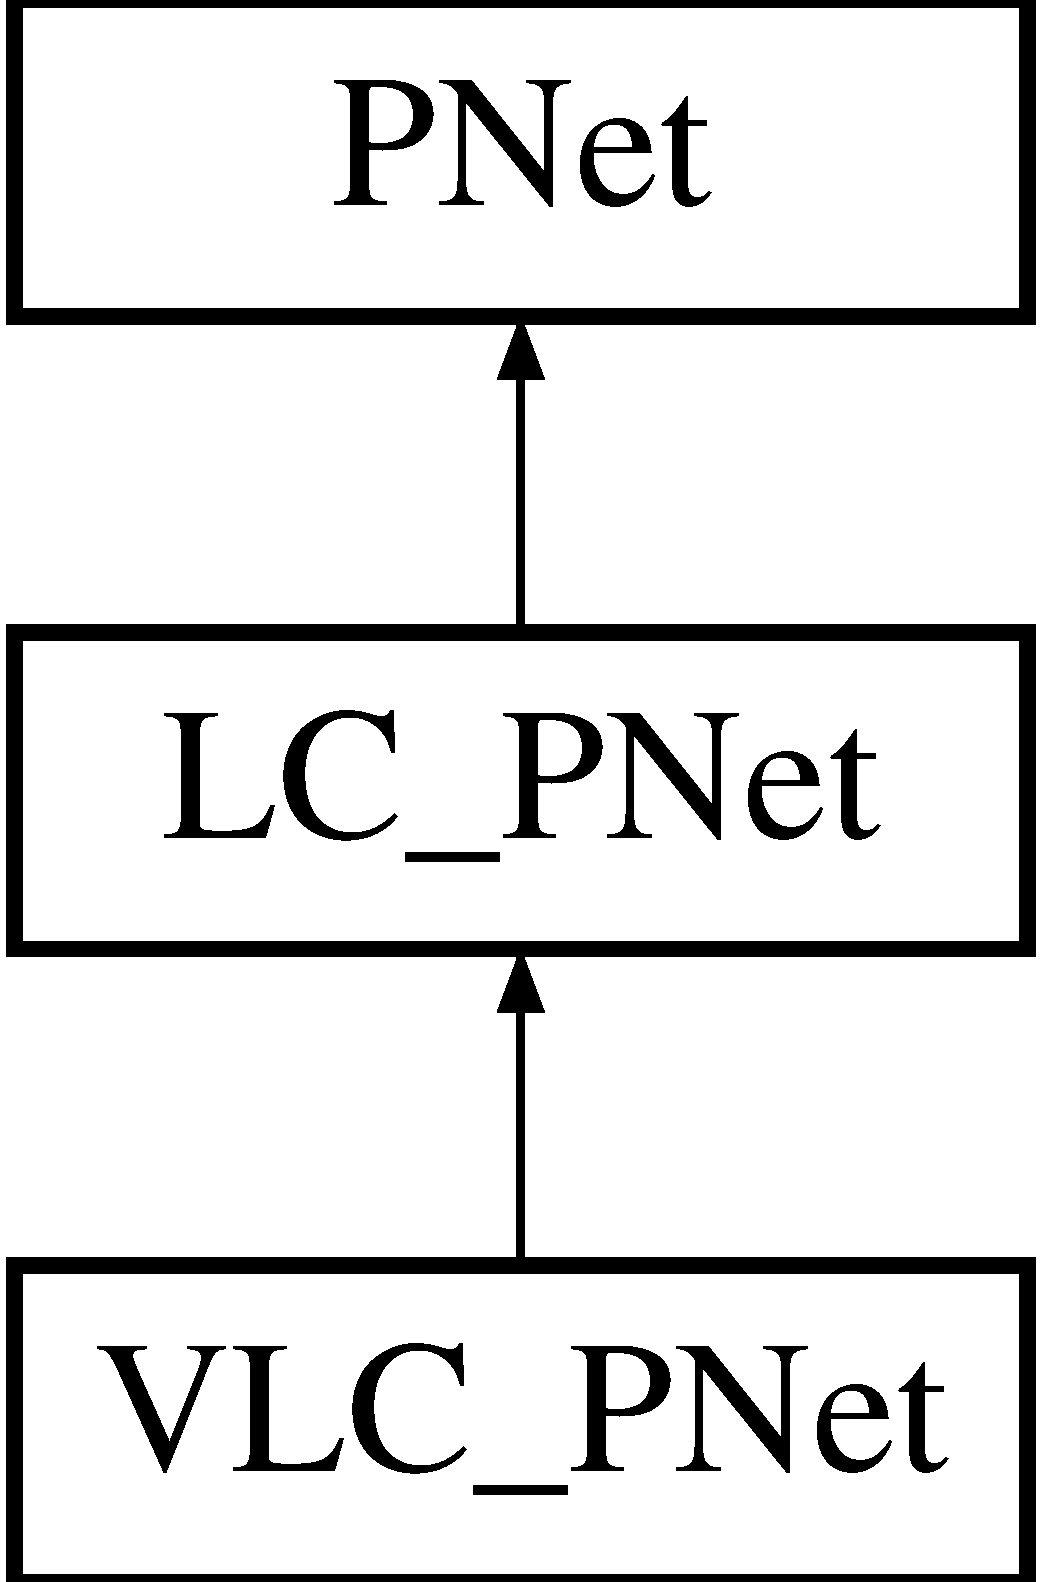
\includegraphics[height=3.000000cm]{classVLC__PNet}
\end{center}
\end{figure}
\subsection*{Public Member Functions}
\begin{DoxyCompactItemize}
\item 
{\bfseries V\+L\+C\+\_\+\+P\+Net} (const int \&N, const int \&C, const int \&S)\hypertarget{classVLC__PNet_a4c7e1b428ce72022e20ed2c7c05fc599}{}\label{classVLC__PNet_a4c7e1b428ce72022e20ed2c7c05fc599}

\item 
void {\bfseries start\+\_\+dynamics} (std\+::default\+\_\+random\+\_\+engine \&generator, const int \&p, const int \&tstatus, const int \&nupdates, const int $\ast$xi, const int \&pattern, const \+\_\+\+\_\+fpv \&a, const \+\_\+\+\_\+fpv \&U, const \+\_\+\+\_\+fpv \&w, const \+\_\+\+\_\+fpv \&g, const \+\_\+\+\_\+fpv \&tau, const \+\_\+\+\_\+fpv \&b1, const \+\_\+\+\_\+fpv \&b2, const \+\_\+\+\_\+fpv \&b3, const \+\_\+\+\_\+fpv \&beta, const int \&tx)\hypertarget{classVLC__PNet_a8df456c85a7e6a0319a14c18f014a7d4}{}\label{classVLC__PNet_a8df456c85a7e6a0319a14c18f014a7d4}

\end{DoxyCompactItemize}
\subsection*{Private Member Functions}
\begin{DoxyCompactItemize}
\item 
void {\bfseries update\+\_\+rule} (const int \&unit, const int \&pattern, const \+\_\+\+\_\+fpv \&U, const \+\_\+\+\_\+fpv \&w, const \+\_\+\+\_\+fpv \&g, const \+\_\+\+\_\+fpv \&tau, const \+\_\+\+\_\+fpv \&b1, const \+\_\+\+\_\+fpv \&b2, const \+\_\+\+\_\+fpv \&b3, const \+\_\+\+\_\+fpv \&beta, const int \&tx, const int \&t)\hypertarget{classVLC__PNet_a59ab7988f2180850a5cb8c74b89a0946}{}\label{classVLC__PNet_a59ab7988f2180850a5cb8c74b89a0946}

\end{DoxyCompactItemize}
\subsection*{Additional Inherited Members}


The documentation for this class was generated from the following files\+:\begin{DoxyCompactItemize}
\item 
/home/deathquasar/\+Projects/\+M\+H\+P\+C/\+Thesis/\+Code/\+Potts\+\_\+code/include/vlc\+\_\+pnet.\+h\item 
/home/deathquasar/\+Projects/\+M\+H\+P\+C/\+Thesis/\+Code/\+Potts\+\_\+code/lib/vlc\+\_\+pnet.\+cpp\end{DoxyCompactItemize}

%--- End generated contents ---

% Index
\backmatter
\newpage
\phantomsection
\clearemptydoublepage
\addcontentsline{toc}{chapter}{Index}
\printindex

\end{document}
